\documentclass[12pt,twoside,english]{article}
\usepackage[utf8]{inputenc}

%%%%%%%%%%%%%%%%%%%%%%%%%%%%%%%%%%%%%%%%%%%%%%%%%%%%%%%%%%%%%%%%%%%%%%%
%% template for II2202 proposal
%% original 2020.08.28
%% revised  
%%%%%%%%%%%%%%%%%%%%%%%%%%%%%%%%%%%%%%%%%%%%%%%%%%%%%%%%%%%%%%%%%%%%%%%
%

%%% Local Variables:
%%% mode: latex
%%% TeX-master: "."
%%% End:

%%TC:ignore
\usepackage[paper=a4paper,dvips,top=1.5cm,left=1.5cm,right=1.5cm,
    foot=1cm,bottom=1.5cm]{geometry}


\usepackage{todonotes}          %to provide inline and margin notes
%\usepackage[T1]{fontenc}
%%\usepackage{pslatex}
\renewcommand{\rmdefault}{ptm} 
\usepackage{mathptmx}
\usepackage[scaled=.90]{helvet}
\usepackage{courier}
%
\usepackage{bookmark}

\usepackage{fancyhdr}
\pagestyle{fancy}

%%----------------------------------------------------------------------------
%%   pcap2tex stuff
%%----------------------------------------------------------------------------
 %%\usepackage[dvipsnames*,svgnames]{xcolor} %% For extended colors
 %%\usepackage{tikz}  %% Already loaded
 %%\usetikzlibrary{arrows,decorations.pathmorphing,backgrounds,fit,positioning,calc,shapes}

%% \usepackage{pgfmath}	% --math engine
%%----------------------------------------------------------------------------
%% \usepackage[latin1]{inputenc}
\usepackage[utf8]{inputenc} % inputenc allows the user to input accented characters directly from the keyboard
\usepackage[english]{babel}
%% \usepackage{rotating}		 %% For text rotating
\usepackage{array}			 %% For table wrapping
\usepackage{graphicx}	                 %% Support for images
\usepackage{float}			 %% Suppor for more flexible floating box positioning
\usepackage{color}                       %% Support for colour 
\usepackage{mdwlist}
%% \usepackage{setspace}                 %% For fine-grained control over line spacing
%% \usepackage{listings}		 %% For source code listing
%% \usepackage{bytefield}                %% For packet drawings
\usepackage{tabularx}		         %% For simple table stretching
%%\usepackage{multirow}	                 %% Support for multirow colums in tables
\usepackage{dcolumn}	                 %% Support for decimal point alignment in tables
\usepackage{url}	                 %% Support for breaking URLs
\usepackage[perpage,para,symbol]{footmisc} %% use symbols to ``number'' footnotes and reset which symbol is used first on each page
\usepackage[binary-units=true]{siunitx} %% to be able to use binary units
\newcommand{\SIadj}[2]{\SI[number-unit-product={\text{-}}]{#1}{#2}}

%% \usepackage{pygmentize}           %% required to use minted -- see python-pygments - Pygments is a Syntax Highlighting Package written in Python
%% \usepackage{minted}		     %% For source code highlighting

%% \usepackage{hyperref}		
\usepackage[all]{hypcap}	 %% Prevents an issue related to hyperref and caption linking
%% setup hyperref to use the darkblue color on links
%% \hypersetup{colorlinks,breaklinks,
%%             linkcolor=darkblue,urlcolor=darkblue,
%%             anchorcolor=darkblue,citecolor=darkblue}

%% Some definitions of used colors
\definecolor{darkblue}{rgb}{0.0,0.0,0.3} %% define a color called darkblue
\definecolor{darkred}{rgb}{0.4,0.0,0.0}
\definecolor{red}{rgb}{0.7,0.0,0.0}
\definecolor{lightgrey}{rgb}{0.8,0.8,0.8} 
\definecolor{grey}{rgb}{0.6,0.6,0.6}
\definecolor{darkgrey}{rgb}{0.4,0.4,0.4}
%% Reduce hyphenation as much as possible
\hyphenpenalty=15000 
\tolerance=1000

%% useful redefinitions to use with tables
\newcommand{\rr}{\raggedright} %% raggedright command redefinition
\newcommand{\rl}{\raggedleft} %% raggedleft command redefinition
\newcommand{\tn}{\tabularnewline} %% tabularnewline command redefinition

%% definition of new command for bytefield package
\newcommand{\colorbitbox}[3]{%
	\rlap{\bitbox{#2}{\color{#1}\rule{\width}{\height}}}%
	\bitbox{#2}{#3}}

%% command to ease switching to red color text
\newcommand{\red}{\color{red}}
%%redefinition of paragraph command to insert a breakline after it
\makeatletter
\renewcommand\paragraph{\@startsection{paragraph}{4}{\z@}%
  {-3.25ex\@plus -1ex \@minus -.2ex}%
  {1.5ex \@plus .2ex}%
  {\normalfont\normalsize\bfseries}}
\makeatother

%%redefinition of subparagraph command to insert a breakline after it
\makeatletter
\renewcommand\subparagraph{\@startsection{subparagraph}{5}{\z@}%
  {-3.25ex\@plus -1ex \@minus -.2ex}%
  {1.5ex \@plus .2ex}%
  {\normalfont\normalsize\bfseries}}
\makeatother

\setcounter{tocdepth}{3}	%% 3 depth levels in TOC
\setcounter{secnumdepth}{5}
%% Acronyms
\usepackage[acronym, nopostdot]{glossaries}
\glsdisablehyper
\makeglossaries

\renewcommand{\headrulewidth}{0pt}
%%%%%%%%%%%%%%%%%%%%%%%%%%%%%%%%%%%%%%%%%%%%%%%%%%%%%%%%%%%%%%%%%%%%
%% End of preamble
%%%%%%%%%%%%%%%%%%%%%%%%%%%%%%%%%%%%%%%%%%%%%%%%%%%%%%%%%%%%%%%%%%%%

\newacronym{AR}{AR}{augmented reality}

% Keywords command
\providecommand{\keywords}[1]
{
  \small	
  \textbf{\textit{Keywords:}} #1
}

\title{Trade-offs Between Immersion and Energy Consumption With Automatic Naturalistic Lighting in Augmented Reality}
\author{
        \textsc{Stefano Formicola}
            \qquad
        \textsc{Christoph Albert Johns}
        \mbox{}\\
        \normalsize
            \texttt{formico}
        \textbar{}
            \texttt{cajohns}
        \normalsize
            \texttt{@kth.se}
}
\date{\today}


\lhead{II2202, Fall 2020, Period 1-2}
%% or \lhead{II2202, Fall 2020, Period 1}
\chead{Draft Project Report}
\rhead{\date{\today}}

\makeatletter
\let\ps@plain\ps@fancy 
\makeatother

\setlength{\headheight}{15pt}
\begin{document}

\maketitle


\begin{abstract}
\label{sec:abstract}

This research project proposes and tests a method to investigate the effect of automatic naturalistic lighting in \gls{AR} applications on immersion and on energy consumption.
A simple open-source card-matching game is modified to implement and control the corresponding rendering setting as provided by Apple's \gls{AR} \gls{API} RealityKit and tested with a small set of users.
A within-subject research design with a small convenience sample is chosen to measure immersion through the \gls{IEQ} while overall \gls{CPU} usage is monitored and logged for both test conditions in randomized order.
A Mann-Whitney-U-test is used to test for significant differences in immersion and \gls{CPU} usage between both conditions.
The pre-test shows that the proposed method is generally appropriate to test the hypothesized relationships.
For a large-scale study, usability issues of the sample application should be resolved for more reliable measures or another application could be considered.
Additionally, it should be considered whether the \gls{IEQ} should be replaced with a questionnaire that is more specific to \gls{AR} applications.
The preliminary results seem to suggest that immersion is not significantly affected by automatic naturalistic lighting whereas \gls{CPU} usage might be higher for the enabled condition, although a larger scale study is required for a more meaningful account.

\end{abstract}

%TC:ignore
\keywords{Augmented reality, Lighting, Immersion, Energy consumption}
%TC:endignore
\clearpage

\selectlanguage{english}
\tableofcontents

\section*{List of Acronyms and Abbreviations}
\label{list-of-acronyms-and-abbreviations}
\renewcommand{\glossarysection}[2][]{} %% skip the title
\printglossary[type=\acronymtype, nonumberlist]

\clearpage
\section{Introduction}
\label{sect:introduction}

% What is the problem?
Through the dissemination of powerful and easy-to-use \glsplural{API}, increasingly advanced features for \gls{AR} have become readily available to developers and designers.
Apple's \gls{AR} \gls{API} \textit{RealityKit}, for example, has enabled creators to easily add occlusion, video textures, and shared states for collaborative experiences to their \gls{AR} applications~\cite{apple_realitykit_2020-1}.
One of the especially notable features has been real-time light estimation~\cite{apple_arlightestimate_2020}.
Applications that enable this feature gain access to information about a scene's lighting with every video frame that is delivered to the current session~\cite{apple_arlightestimate_2020}.
This information can then be used to apply dynamic shading to virtual objects matching the real-world lighting conditions~\cite{apple_arlightestimate_2020}.
Apple's RealityKit \gls{API} enables this feature by default and-–depending on the available hardware–-uses one or multiple probes in the scene to measure and estimate this so called "environment lighting"~\cite{apple_disablearenvironmentlighting_2020}.
The resulting lighting estimate is then applied to the virtual objects in the scene~\cite{apple_disablearenvironmentlighting_2020}.
To achieve this naturalistic lighting, camera-sensor data is continuously processed to estimate and approximate the environment's lighting conditions in order to dynamically add the appropriate shading to each virtual object~\cite{apple_arlightestimate_2020,apple_disablearenvironmentlighting_2020}.
Depending on the scene and lighting conditions, this can be a computationally intensive process~\cite{steed_constructing_2016}.
Enabling automatic naturalistic lighting could, therefore, lead to increased scene realism at the cost of decreased energy efficiency.

This research aims at illuminating the relationship between immersion and energy consumption in deploying automatic naturalistic lighting, thus empowering developers and designers to decide the most appropriate feature sets for their applications considering both user experience and sustainability aspects.
For this, our project builds on two main lines of research: prior works evaluating the relationship between visual characteristics of \gls{AR} objects and user experience (e.g.~\cite{gabbard_effects_2006}) and research on the approximation of natural lighting conditions within virtual scenes in augmented reality (e.g.~\cite{aittala_inverse_2010}).
While there has been extensive research on the effect of design decisions on several aspects of user experience in digital games~\cite{johnson_validation_2018} -- even in \gls{AR} games in a few instances (e.g.~\cite{georgiou_development_2017}) -- the effect of lighting and more specifically automatic naturalistic lighting in \gls{AR} games on immersion seems not to have been examined yet.

We chose to investigate the effect of automatic naturalistic lighting on immersion--in contrast to, for example, \textit{flow}~\cite{csikszentmihalyi_flow_1990}--, because it is independent from optimal experience, which our method will not be able to produce, and very likely to relate to visual presentation and, therefore, lighting~\cite{jennett_measuring_2008}.
There exist multiple alternative measures that could have been chosen to explore aspects of the experience when playing video games instead (see~\cite{dey_systematic_2018, dunser_survey_2008} for overviews).
We reason, however, that immersion is an appropriate measure for this study since automatic naturalistic lighting is likely to enhance the sense of realism of a scene and might therefore affect users' sense of immersion.
As Witmer and Singer argue, "scene realism" is one of the governing factors for presence in virtual environments~\cite{witmer_measuring_1998}, which in turn affects how immersive a virtual environment appears~\cite{jennett_measuring_2008}.

Since we are limited by our resources in terms of time and budget, however, and since this research project is conducted during the COVID-19 pandemic, we will not be able to reach the necessary number of participants that would be required to fully illuminate said relationship.
Instead, we will focus on preparing a full-scale study by proposing and pre-testing the study design as well as developing and evaluating the necessary tools, for example a sample application and an analysis script.
This project will, therefore, give some indication about the results of a full-scale study, but will mainly provide insights into the strengths and weaknesses of our chosen method and tools.
The expected deliverables for our project are: an example \gls{AR} application to measure immersion levels and monitor energy consumption; a pre-tested and evaluated method (setup, procedure, and analysis) for a full-scale study; and an indication for the results of a full-scale study.


% What are the research questions?
Overall, we propose to explore the following questions:

\begin{description}
    \item[RQ1.] Do users perceive a difference in immersion between enabled and disabled automatic naturalistic lighting?
    \item[RQ1a.] If they perceive a difference, are the participants able to tell that lighting is the cause?
    \item[RQ2.] How does enabling automatic naturalistic lighting affect \gls{CPU} usage?
\end{description}

In our pre-test, energy consumption will be measured in terms of \gls{CPU} usage for two major reasons.
First, because there is no dedicated \gls{GPU} in the mobile device we will be testing, so the \gls{CPU} will handle all processing related to the \gls{AR} experience.
And second, because CPU usage can very finely be measured on the test device in contrast to general energy consumption.

While we are aware that we will only be able to test the proposed method on a small scale, we hypothesize the following outcomes for a full-scale experiment:

\begin{description}
    \item[H1.] Users experience higher immersion levels when automatic naturalistic lighting is enabled.
    \item[H1a.] Users are able to tell that the lighting was different between both runs of the experiment.
    \item[H2.] \gls{CPU} usage is higher when automatic naturalistic lighting is enabled.
\end{description}

As has been explained above, scene realism is positively correlated with presence and thereby immersion.
That is why we expect the lighting condition that more closely matches the scene's natural environment to lead to higher levels of immersion, resulting in the first hypothesis.
Second, because the difference between both conditions lies in a salient visual feature which affects \gls{AR} objects' color and reflections, we expect not only the indirect measure of immersion as assessed through the \gls{IEQ} to be affected.
We instead hypothesize that users will recognize the difference between both conditions and will be able to articulate how they differ without support from the examiner.
And finally, regarding the energy impact of automatic naturalistic lighting, we expect the computationally intensive continuous probing and estimation of the \gls{AR} scenes environment lighting to lead to higher levels of overall \gls{CPU} usage.


\section{Method}
\label{sect:method}

We propose a within-subject design to test the effects of the two conditions \textit{automatic naturalistic lighting enabled} and \textit{automatic naturalistic lighting disabled} on immersion using the \gls{IEQ} developed by Jennett et al.~\cite{jennett_measuring_2008} while measuring \gls{CPU} usage via a device metrics logging tool in combination with a sample \gls{AR} application.
For this, we modified an existing open source mobile \gls{AR} game and prepared a form that includes the \gls{IEQ}, while Xcode's Developer Tools' \textit{Instruments} were used to measure \gls{CPU} usage over time.
Because of its popularity across countries and languages, we considered the game \textit{Memory} or \textit{Concentration}, in which players have to remember the order and color of different cards, a valid candidate for the experiment.
The implementation was done for iOS devices and developed on Apple's \gls{IDE} Xcode using the ARKit and RealityKit \glsplural{API}.
The user interface included a toggle button hidden from the player to enable and disable the automatic naturalistic lighting feature for the two runs of the experiment (see Figure \ref{fig:sample_app_comparison} for a comparison between enabled and disabled automatic naturalistic lighting in the sample application).
The experiment consisted of one three-minute session of gameplay for each condition, with and without the automatic naturalistic lighting, per subject.
In the following, the targeted participant profile, procedure, data collection, and analysis are described.

\begin{figure}[h]
    \centering
    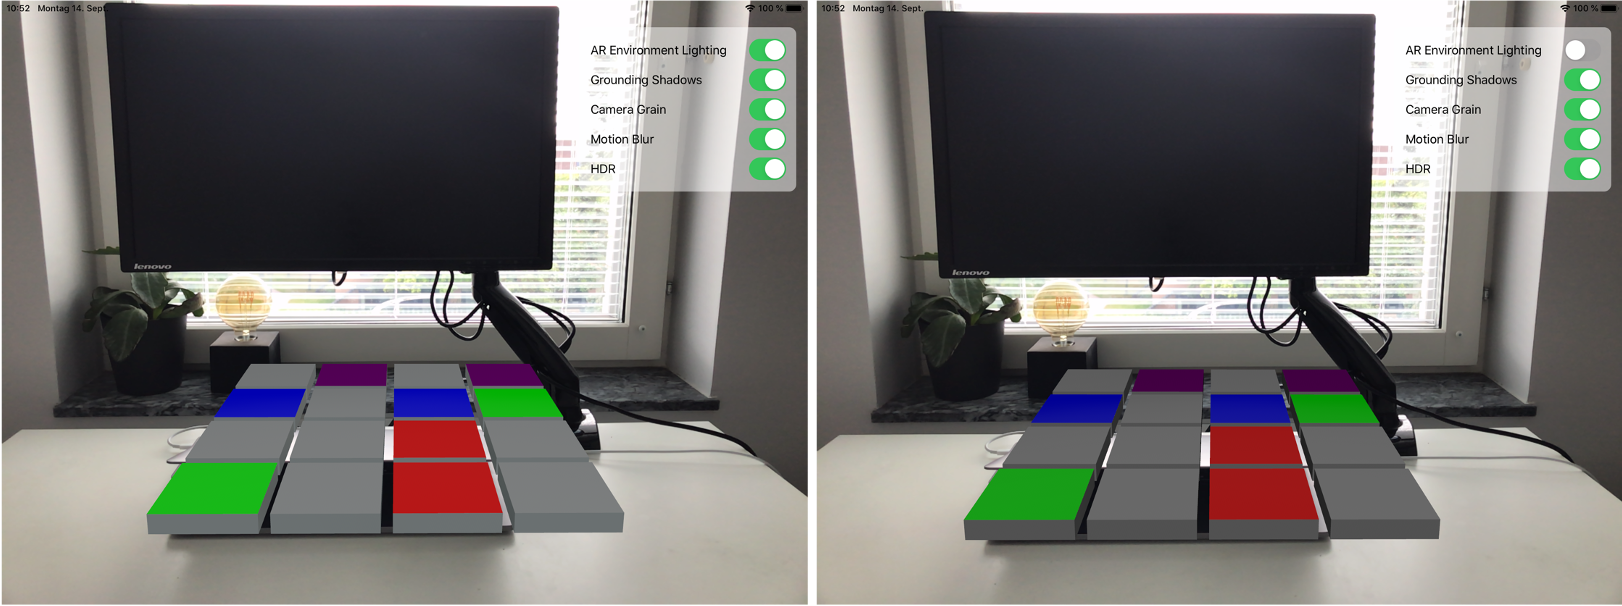
\includegraphics[width=0.7\textwidth]{imgs/sample_app_comparison.png}
    \caption{Comparison between enabled (left) and disabled (right) automatic naturalistic lighting in the sample card-matching \gls{AR} application. The controls can be hidden before the test device is handed over to the participant.}
    \label{fig:sample_app_comparison}
\end{figure}

\subsection{Participants}
\label{sect:participants}

The participants were recruited via an opportunity sample and were--due to the difficulties and restrictions regarding gatherings of people during the COVID-19 pandemic--mostly international students living at KTH Main Campus.
To limit the effect of novelty on immersion levels, participants were required to have had played a card-matching game similar to the sample game before.
It was, however, not required that they have played a digital version of this game before taking part in the experiment.
To further mitigate the effect of novelty, participants were required to have experienced an \gls{AR} scene on a mobile handheld device before.
Overall, seven participants took part in this study.
They had an average age of 24.7 (SD = 1.60), ranging from 23 to 28 years.
All seven participants were male.

\subsection{Procedure}
\label{sect:procedure}

We modified an open-source \gls{AR} card-matching game~\cite{cobb_maxxfrazerrealitykit-cardflip_2020} to include an option to enable and disable automatic naturalistic lighting using RealityKit's \textit{.disableAREnvironmentLighting} render option for a repeated measures study design.

Before the start of the experiment participants were informed about the collection of data regarding the device activity and their questionnaire answers after both runs of the game.
Moreover, their right to withdraw from the experiment at any time was clarified as well as the possibility to ask for the deletion of all data associated with their person.
The purpose of the experiment was stated to the participants in general terms as "investigating immersion in \gls{AR} games" to avoid influencing their perception of the scene by directing their attention towards lighting. 
They were asked to fill a consent form in a Google Forms document (see Appendix \ref{sect:consent-form}).

The game was presented to participants on an Apple iPad Pro 2017 (model number FPDY2FD/A) in an indoor setting with controlled lighting where participants were asked to complete as many rounds of the card-matching game for each of the two lighting conditions as they could, before they were interrupted after three minutes and the render option was changed for the second run.
The order of both render options was randomized to improve reliability and participants were not informed about the currently active render option to avoid biases.

The sample application was chosen due to its simplicity in functionality and visual presentation as well as general familiarity, thereby reducing the risk of errors in use or unwanted effects on immersion due to scene complexity or novelty.
To further mitigate this risk and to address the concerns brought up by Jennett et al.~\cite{jennett_measuring_2008} regarding the effect of prior experience on immersion, participants were given a trial period with a third lighting condition: disabled automatic naturalistic lighting and an added point light above the scene.
The goal stated to the participants was to complete as many rounds of the game as possible and with as few errors as possible, following the study design of Jennett et al.~\cite{jennett_measuring_2008}.
The goal of this decision was to allow for a more challenging experience across player ability levels, thereby increasing flow~\cite{csikszentmihalyi_flow_1990} and general immersion levels as well as reducing overall variance in immersion~\cite{jennett_measuring_2008}.
The first run was considered started after the participants indicated that they were ready for the experiment to begin.
After the experiment, participants were debriefed and fully informed about the purpose of the study and given the opportunity to withdraw their consent.
The duration of the experiment per participant was around twenty minutes.

\subsection{Data collection}
\label{sect:data_collection}

During each run of the experiment, the \gls{IDE} Xcode and more specifically its \textit{Instruments} feature~\cite{apple_xcode_2020} were used to log the test device's \gls{CPU} utilization in three second intervals, according to Apple's type definitions~\cite{apple_system_2020}.
While there exists a more general power metric that can be logged through the same application~\cite{apple_energy_2020-1}, that metric is discrete and too unspecific to be elastic towards enabled and disabled automatic naturalistic lighting and was, therefore, not used.
We decided not to have participants think aloud during their app usage to avoid unwanted effects on their experience and, thus, immersion~\cite{van_den_haak_retrospective_2003}.
After each run, participants were asked to fill out the \gls{IEQ} (see Appendix \ref{sect:ieq}) to measure their levels of immersion dependent on the lighting treatment.
After the second run, participants were additionally asked about their general experience using the application and to elaborate on any differences they noticed between both runs.
While alternatives such as tracking eye movement or measuring reaction times could also have been used to measure immersion~\cite{jennett_measuring_2008}, we chose a questionnaire approach as the most economical option that still has satisfactory precedence in literature~\cite{boyle_engagement_2012}.
If a participant referred to "light", "lighting", "color", or "contrast" while answering these open questions, the difference in lighting was considered as noticed by the user.

\subsection{Data analysis}
\label{sect:data_analysis}

After the above data had been successfully gathered, we used a Jupyter Notebook with Python~3.8.3 to conduct a statistical analysis regarding the participants' immersion levels and the \gls{CPU} usage between both lighting conditions using a Mann-Whitney U-test to check for significant differences.
We chose this test because it does not require a normal distribution and because it was used by Jennett et al. in their original experiments~\cite{jennett_measuring_2008}.
However, the Student's \textit{t}-test's could also have been used if the data was normally distributed as for example Nordin et al.~\cite{nordin_attention_2013} do in their immersion experiments.
Additionally, we report the results of the open questions.

We were aware that neither the results of our analysis of variance nor those of our qualitative research should be used to infer knowledge about either the effect of automatic naturalistic lighting on immersion or energy consumption due to the small sample size.
Rather, the analysis was carried out in order to evaluate the chosen methods and to illustrate how such analysis should have been done if the same study was carried out on a larger scale and to give some indication as to the results of such a full-scale study.

\section{Results}
\label{sect:results}

Our results can be divided into three parts: (1) the indicative results of our statistical analysis, (2) our own observations when developing and using the tools we devised, (3) our observations of the study participants, and (4) the feedback and comments of our study participants.
Since the main contribution of this study lies in the tooling that we developed and pre-tested for a full-scale study, let us first let us at the secondary contribution: the indicative results of our statistical analysis.

All statistical analysis was performed using Python 3.8.3 with the packages Pandas 1.1.4 and SciPy 1.5.4.
All visualizations were created using Seaborn 0.11.0.
The immersion scores per question according to the \gls{IEQ} were calculated as ranging from a 1 for strongly disagree to a 5 for strongly agree.
Scores for positively formulated questions were added, while scores for negatively formulated questions were subtracted to calculate the overall immersion score per participant and condition.
Overall \gls{CPU} usage per timestamp was calculated by adding the \gls{CPU} usage percentages for all activity kinds with the same timestamp.
Since the System CPU Percentage Engineering Type~\cite{apple_system_2020} has a range from 0\% to 100\% multiplied by the number of \gls{CPU} cores in the given device, this can result in values exceeding 100\% (or 1 as in the formatting of our analysis).
Contrary to our first hypothesis \textbf{H1}, overall immersion scores did not differ significantly between both conditions (Mann-Whitney $ U = 18.5 $, $ p = 0.241 $) with the mean overall immersion score for the automatic naturalistic lighting disabled condition even slightly exceeding the enabled condition with scores of 74.7 (SD = 7.3) and 76.0 (SD = 6.6) respectively (see Figure \ref{fig:immersion_plot}).

\begin{figure}[h]
    \centering
    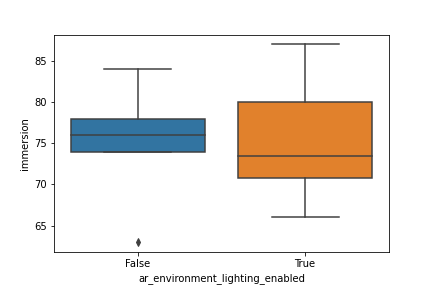
\includegraphics[width=0.5\textwidth]{imgs/immersion_plot}
    \caption{Immersion scores for the disabled and enabled conditions in our small pre-test ($ N = 7 $).}
    \label{fig:immersion_plot}
\end{figure}

Regarding hypothesis \textbf{H1a}, there was no indication whether most participants in a full-scale study would notice a difference between both conditions as three of the seven participants in our pre-test stated they had not noticed any distinction.
Within the group of participants that had answered to have noticed a difference, the immersion scores between automatic naturalistic lighting enabled and disabled did not differ significantly (Mann-Whitney $ U = 4.0 $, $ p = 0.155 $) with mean immersion scores of 76.3 (SD = 4.9) and 76.0 (SD = 11.4) respectively.
Finally, contrary to our hypothesis \textbf{H2}, mean \gls{CPU} usage did not significantly differ between both conditions (Mann-Whitney $ U = 16.0 $, $ p = 0.405 $) with 61.8\% (SD = 6.7\%) mean overall \gls{CPU} usage in the disabled condition and 63.1\% (SD = 6.6\%) in the enabled condition.
However, as can be seen in Figure \ref{fig:cpu_raw_plot}, the distributions of overall \gls{CPU} usage did appear different.
The enabled condition resulted in a significantly higher overall \gls{CPU} usage even in our small pre-test (Mann-Whitney $ U = 53272.5 $, $ p < 0.05 $).

\begin{figure}[h]
    \centering
    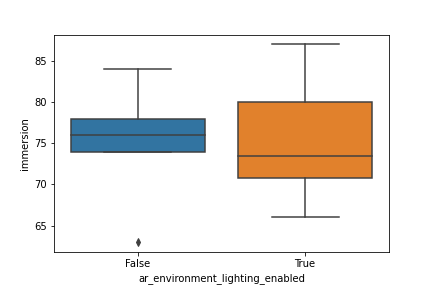
\includegraphics[width=0.5\textwidth]{imgs/cpu_raw_plot}
    \caption{Overall \gls{CPU} usage for the disabled and enabled conditions in our small pre-test ($ N = 7 $). The overall \gls{CPU} usage can exceed 1 for devices with more than one \gls{CPU} core (range from 0 to number of cores) as specified in the corresponding data type definition of the logging software~\cite{apple_system_2020}.}
    \label{fig:cpu_raw_plot}
\end{figure}

While conducting the pre-test, we experienced some difficulties with our chosen software.
The modified sample application as well as the monitoring and logging software chosen had reliability issues that hindered the data gathering process.
In one of the experiments, logging of the \gls{CPU} usage suddenly stopped after circa 1.5~min.
While other data such as network events that were logged automatically by the software could still be accessed, \gls{CPU} data was non-retrievable.
In another experiment, the logging software crashed after requesting to stop and save the recording.
Here again, the \gls{CPU} data wan non-retrievable.
The sample application, similarly, experienced some issues that seemed to relate to the Xcode \gls{IDE}.
In one experiment, the application failed to exit through the software and had to be manually shut down.
Regarding less severe concerns, the sample application appeared to lack in terms of its feedback mechanisms.
During multiple experiments, the probing phase (i.e. the phase during which the application gathers information about the environment, specifically to find a horizontal plane to use as an anchor for the virtual objects of the scene) which was indicated by an overlay with instructions to slowly move the device was exited without placing the virtual objects in an appropriate time frame.
No inherent error or pattern to this behavior could be identified.
This lead to multiple restarts of the application which delayed several runs of the experiment.
The Google Forms questionnaire developed for data gathering did not pose any significant challenges when used by the testers.
The Jupyter notebook developed for data analysis, similarly, did not lead to any significant difficulties.

During the experiments, several participants experienced difficulties when interacting with the sample application.
Since the application does support scaling and positioning during the setup phase for increased usability but does not save these settings, the virtual cards were displayed in the original scale and position after each successful game resulting in visible irritation by the participants.
Additionally, the participants seemed to experience some discomfort holding the test device as multiple participants started frequently adjusting their grip during the second run of the experiment.
One participant even rested the device on a table to avoid having to hold it.
It was, furthermore, noticeable that all participants moved the device during the trial phase of the experiment and some at the beginning of the first run, but all stopped moving the device altogether eventually.
They instead remained in a fixed position once a comfortable posture was discovered and only interacted with the application by tapping the screen.
One participant tried multiple different postures, positions, distances, and orientations during the trial phase but, just as the other participants, stopped this exploratory behavior completely once the first run started.
Finally, multiple participants were briefly distracted during one or both runs of the experiment by noises or other people in the test environment.
One participant attempted to start a conversation with the testers during one of the runs which was denied but still interrupted the run.

Our discussions with the participants revealed that the reliability and usability issues we observed matched the participants' experiences.
Multiple participants noted that they were irritated by the inconsistent scale and position of the virtual objects.
Three participants stated unprompted that the device was uncomfortable to hold for the duration of the experiment due to its size and sharp edges.
The sample application was generally accepted.
Two participants noted that its simplicity might limit the potential immersion and that the lack of more complex objects and reflections might result in generally smaller differences in immersion between both runs.
They, furthermore, suspected that this would make it harder for participants to notice any differences between both runs.
The results would additionally be affected by the study design itself.
Some participants noted that asking about the overall experience and any differences between both runs of the experiment would lead to biased answers since it provoked answers even if the participant would not have experienced significant differences.
One participant suggested a third experiment variation in addition to the randomized order where the active render setting is not changed between both runs.

\section{Discussion}
\label{sect:discussion}

Since the goal of this project is to develop and evaluate a method and the corresponding tools for a full-scale study on the effects of automatic naturalistic lighting on immersion and energy consumption, it needs to be established how well the proposed method is able to provide insight into both relationships and which shortcomings still need to be overcome.
For this, the observations and comments above need to be consolidated into actionable insights.
In the following, the two major phases of the envisioned full-scale study will be evaluated separately in regards to how well the developed method and tools are suited to meet each step's requirements: (1) data gathering and (2) data analysis.

The data gathering process as proposed makes use of the sample application developed in this project, the associated logging software, and the Google Forms form that includes the \gls{IEQ}.
As described in Section \ref{sect:method}, these tools are used in a within-subjects study design with a trial run and two test conditions in randomized order pre-tested with a small convenience sample.
While the proposed method was generally appropriate to gather the required data, each of the tools as well as the study design itself has several weaknesses that should be addressed before a full-scale study is conducted.
First, regarding the general setup, we noticed some inconsistencies in how the experiment was run that might affect the results in a full-scale study.
Since we did not have access to one consistent room with minimal distractions for our testing, we conducted the pre-test in multiple environments with various lighting conditions and possible disturbances.
This was especially noticeable when multiple participants were in the same room or when a common room was used.
The distractions caused by these surroundings and the inconsistencies in the data that might be caused by the different lighting conditions should be avoided in a full-scale study by using a consistent laboratory room with controlled lighting and minimal distractions.
Additionally, we experienced some difficulties with the sample application and the runs of our experiment.
As some participants noted, the test device was rather uncomfortable to hold for longer periods of time which might have affected the general lack of movement we observed.
In an \gls{AR} application, it could be argued that users should move to immerse themselves in the experience provided which our sample application failed to motivate.
Instead, most participants stood still for the entire experiment which might have lead to generally too low immersion levels to find a difference between both tested conditions.
Furthermore, we experienced difficulties regarding the application's reliability and stability, as it as well as the associated logging tool crashed twice at such a crucial moment that the experiments' data was non-retrievable.
In addition, some less severe usability concerns should be considered before using the sample application in larger setting.
The application currently requires the tester to manually adjust the render setting (i.e. enabling or disabling automatic naturalistic lighting) which can easily lead to errors and thereby faulty data.
It also does not preserve state about the position and scale chosen by the user which further demotivates movement.
Moreover, as one participant noted, the virtual scene might be lacking in complexity resulting in a less noticeable difference between both tested conditions.
While it could be argued that the game's visual complexity is a realistic representation of the complexity of most current \gls{AR} applications, this claim is yet to be supported by additional research.
To conduct the experiment in a full-scale study, these issues should be addressed and fixed, for example by considering a different device (e.g. a phone), a different framework (e.g. Unity), or an adjusted application (e.g. using different forms and materials in the virtual scene).

Regarding the questionnaire that accompanied the experiment, there are four observations that we want to highlight here.
First, we noticed that multiple participants were slightly irritated by the fact that we used one Google Forms form for all information regarding one experiment (incl. the consent form and data to be filled by the tester).
This interrupted the flow of the experiment and can easily be avoided by splitting the questionnaire into one to be filled by the participant and one to be filled by the tester which can be joined by an anonymous and random ID.
Second, we observed that some participants might have been affected in their answers to the \gls{IEQ} by our presence in the room when they filled the questionnaire.
Two participants, for example, asked for an explanation of one of the questions of the \gls{IEQ}.
In order to not affect the results of the questionnaire, the participants should answer the questions to the best of their knowledge and understanding.
One simple way to mitigate this problem would therefore be to leave the room where the experiment is being conducted for duration of the questionnaire.
Third, we became aware of the fact that our definition for the question whether a participant had noticed a difference between both tested conditions was too wide and therefore might have lead to some inconsistencies in understanding.
This might have influenced the results of our analysis regarding hypothesis \textbf{H1a}, since we did not find any clear indication whether users would or would not notice the difference in lighting.
For a full-scale study, this question should be further defined and included in the form to be answered by the participant.
Finally, and related to the point above, the choice of the \gls{IEQ} might want to be re-considered since some of the questions (e.g. To what extent was your sense of being in the game environment stronger than your sense of being the real world?) are less suited for an \gls{AR} game.
This might be one of the reasons, why our preliminary results regarding \textbf{H1} seem to indicate no significant effect of automatic naturalistic lighting on overall immersion.
Since there are alternatives available that are in some cases even developed specifically for \gls{AR} applications~\cite{georgiou_development_2017}, these should be reviewed before conducting a full-scale study based on the \gls{IEQ}.

In regard to the overall study design, the lack of a clear script or protocol to explain the experiment in detail and consistently to each participant became clear when multiple participants stopped after their first completed run of the sample game during the first tested condition.
Despite the explanations given by the testers, they were unaware that their goal was to complete as many runs of the game with as few errors as possible within the given time frame.
This shows that the explanations were unable to provide the participants with the necessary information about their task during the experiment.
For a full-scale study, a clear protocol to be read aloud by the tester should be considered.
Moreover, as one participant pointed out, the inclusion of a placebo condition might be an appropriate addition to further control bias.
While the randomization is well suited to reduce the effect of order on the overall immersion scores, introducing a condition where participants are shown the same lighting in both conditions could reveal further information about the effect that simply asking for immersion twice and asking for difference at the end of the experiment might have on the results.

This brings us to the second phase of a potential full-scale experiment, the data analysis.
While the Jupyter notebook developed during this project is generally suitable to process and analyze the gathered data, some of the decisions about the analyzed measures and the meaning that can be derived from their results can be put into question.
One minor feature that is missing from the notebook at this stage is a test for normality and the subsequent Student's t-test that might be able to provide some additional insight into the effect of automatic naturalistic lighting on immersion and \gls{CPU} usage.
On a more severe note, it can be argued that \gls{CPU} usage is unsuitable to measure energy consumption since it is not examined both truly correlate, since, typically, the \gls{GPU} handles most computation for rendering, and since overall \gls{CPU} usage is not only affected by the sample application.
Multiple background services might mask the effect of automatic naturalistic lighting on the \gls{CPU}.
While the measure was chosen, among other reasons, because of its granular logging possibilities and while it seems to be affected by the rendering condition in our preliminary testing (see the analysis regarding \textbf{H2} in Section \ref{sect:results}), these concerns should be addressed by further researching and considering alternative measures and frameworks as well as testing those measures chosen for their correlation with more direct but less granular measures of energy consumption like Instrument's Abstract Power Measurement~\cite{apple_abstract_2020}.
Finally, it should be reviewed whether the study design and tooling provided by this project is economical enough for a full-scale study.
Since the setup requirements are quite high--a consistently available, non-distracting room with controlled lighting, a consistent test device, at least one tester per participant, and both a questionnaire as well as an experiment-- and since the results might be fast outdated due to the fast-changing API and underlying technology (e.g. the camera or processor), a full-scale study might consider splitting off or re-designing parts of the study, for example by testing the effect of automatic naturalistic lighting on energy consumption in a separate, more controlled study without participants or by including multiple devices and API versions in the study to test for their effect on the results.

Overall, the proposed method and tools are suitable to conduct a full-scale study on the effects of automatic naturalistic lighting on immersion and energy consumption, but each of the parts should carefully be considered, evaluated, and possibly modified before investing heavily in such an endeavor.


\bibliography{II2202-proposal}
% \bibliographystyle{IEEEtran}
\bibliographystyle{myIEEEtran}

\appendix
\section{Appendix: Immersive Experience Questionnaire}
\label{sect:appendix}
\label{sect:ieq}
\subfile{lib/ieq}
\section{Appendix: Participants' Consent Form}
\label{sect:consent-form}
\subfile{lib/consent-form}
\clearpage
\end{document}
